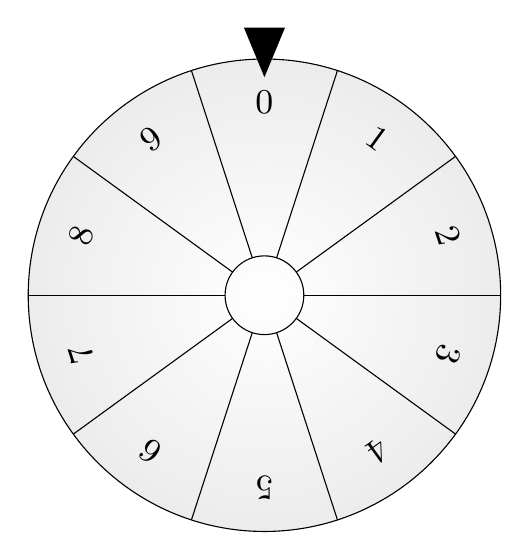
\begin{tikzpicture}
  \usetikzlibrary{shapes.geometric}
  \node at (0, 0) {};

  \pgfmathsetmacro{\radius}{3.}
  \pgfmathsetmacro{\innerradius}{0.5}
  \pgfmathsetmacro{\labelradius}{2.45}
  % adding a subtle gray tone to add a bit of "personality"
  \shade[shading=radial, inner color=white, outer color=gray!15] (0,0) circle (\radius);
  \draw (0,0) circle (\radius);
  \draw (0,0) circle (\innerradius);
  % main lines
  \foreach \x in {0, 36,...,359} \draw (\x:\innerradius) -- (\x:\radius);
  % labels and longer lines at every 10 degrees
  \foreach \x in {0,...,9}
  {
    \node[scale=1.4, rotate=\x*-36] at (360-\x*36+90:\labelradius) {{\small\x}};
    %\draw (\x:\tendegrad) -- (\x:\radius);
  };
  \node[isosceles triangle, draw, fill=black, minimum size=0.5cm, rotate=270] (T) at (0,\radius+0.25){};
\end{tikzpicture}
